\documentclass[../main.tex]{subfiles}

\begin{document}
\chapter{The Nash Model}
\begin{definition}[Nash equilibrium profile]
    A two-player Nash equilibrium profile for $(X,Y, f: X \times Y \to \mathbb{R}, g: X \times Y \to \mathbb{R})$ is a pair $(\overline{x}, \overline{y}) \in X \times Y$ such that:
    \begin{itemize}[noitemsep]
        \item $f(\overline{x}, \overline{y}) \geq f(x, \overline{y})$ for all $x \in X$
        \item $g(\overline{x}, \overline{y}) \geq g(\overline{x}, y)$ for all $y \in Y$
    \end{itemize}
    A Nash equilibrium profile (\gls{NEp}) is a joint combination of strategies, which is stable w.r.t. unilateral deviations of any individual player.
\end{definition}
At equilibrium, neither player can improve her utilities by changing strategy.

In fact, it is not even convenient for the players to change, given that each one takes for granted that the other one will play the selected strategy.

\begin{example}[Prisoner's Dilemma]
    Recall that in this game higher utility means \textit{more years in prison}, so one wants to minimize utilities: to find Nash equilibria one needs to replace $\geq$ with $\leq$
    \[
        \begin{pmatrix}
            (5,5) & (0,7) \\
            (7,0) & (1,1)
        \end{pmatrix}
    \]
    The Nash equilibrium is given by $\overline{x} = x_1$ and $\overline{y} = y_1$. For,
    \begin{itemize}
        \item $f(x_1, y_1) = 5 \leq f(x_2, y_1) = 7$
        \item $g(x_1, y_1) = 5 \leq g(x_1, y_2) = 7$
    \end{itemize}
    \begin{note}
        One could find even the (unique) Nash equilibrium $(5,5)$ by means of the Principle of Dominated Strategies: since $5 < 7$ and $0 < 1$
        \begin{itemize}
            \item the second row is strictly dominated by the first one
            \item the second column is strictly dominated by the first one
        \end{itemize}
    \end{note}
\end{example}

The main ideas of the Nash model can be seen with two players: having more players does not add complexity to the concept (except for the notation).

\begin{definition}[Nash equilibrium (general)]
    Let us consider a $n$-player game with strategy sets $X_i$ for each player and payoffs $u_i: X \to \mathbb{R}$ with $X = \prod_{i=1}^n X_i$.

    Let $x = (x_1, \ldots,x_{i-1}, x_i, x_{i+1} ,\ldots, x_n)$ be a strategy profile.

    Let $x_{-i} = (x_1, \ldots, x_{i-1}, x_{i+1}, \ldots, x_n)$ be the strategy profile of all players except player $i$.

    We can write $x = (x_i, x_{-i})$ to emphasize the role of $x_i$.

    Then $\overline{x} = (\overline{x}_i)^n_{i=1}$ is a Nash Equilibrium if for all $i$, for every $x \in X_i$:
    \[
        u_i (\overline{x}) \geq u_i(x_i, \overline{x}_{-i})
    \]
\end{definition}

\section{New definition of rationality}
The notion of Nash Equilibrium provides a \textbf{new definition of rationality}. But how does it relate to the previous definitions of rationality?

\subsection{Dominant strategies}
Suppose $\overline{x}$ is a \textbf{(weakly) dominant strategy} for Pl1: that is
\[
    f(\overline{x}, y) \geq f(x, y) \quad \forall x \in X, \forall y \in Y
\]
if $\overline{y}$ maximises the function $g(\overline{x}, y)$ for Pl2, then $(\overline{x}, \overline{y})$ is a Nash Equilibrium.
\begin{proof}
    For $\overline{x}$ weakly dominant it is true, in particular, that $f(\overline{x}, \overline{y}) \geq f(x, \overline{y})$ for all $x \in X$, thereby satisfying the first condition of the Nash Equilibrium.

    Then the maximization requirement that $\overline{y}$ be such that $g(\overline{x}, \overline{y}) \geq g(\overline{x}, y)$ for all $y \in Y$ naturally satisfies Nash condition on the utility function $g$ for Pl2.
\end{proof}

\begin{theorem}[Non-uniqueness of Nash Equilibrium]
    Let's suppose that $\overline{y}$ maximises the function $g(\overline{x}, y)$, then:
    \begin{itemize}[noitemsep]
        \item if $\overline{x}$ is a weakly dominant strategy for Pl1, then other Nash Equilibria beyond $(\overline{x}, \overline{y})$ can exist
        \item if $\overline{x}$ is a strictly dominant strategy for Pl1, then $(\overline{x}, \overline{y})$ is the unique Nash Equilibrium
    \end{itemize}
\end{theorem}

\begin{proof}
    Assume that there is another Nash Equilibrium $(\overline{x}', \overline{y}')$ different from $(\overline{x}, \overline{y})$.
    By definition it implies that $f(\overline{x}', \overline{y}') \geq f(\overline{x}, \overline{y}')$. However:
    \begin{itemize}
        \item If $\overline{x}$ is a weakly dominant strategy (so $f(\overline{x}, y) \geq f(x, y)$ $\forall x, y$) this inequality must hold also for the particular case of $\overline{y}'$: $f(\overline{x}, \overline{y}') \geq f(\overline{x}', \overline{y}')$, this is valid assuming $f(\overline{x}, \overline{y}') = f(\overline{x}', \overline{y}')$. Hence $(\overline{x}', \overline{y}')$ can be another Nash Equilibrium.
        \item If $\overline{x}$ is a strictly dominant strategy (so $f(\overline{x}, y) > f(x, y)$ $\forall x, y$) this inequality must hold also for the particular case of $\overline{y}'$: $f(\overline{x}, \overline{y}') > f(\overline{x}', \overline{y}')$ but this cannot be true with the initial assumption of $(\overline{x}', \overline{y}')$ being a Nash Equilibrium. Hence $(\overline{x}, \overline{y})$ is the unique Nash Equilibrium.
    \end{itemize}
\end{proof}
\begin{example}
    Compare the following two zero-sum games:
    \[
        \begin{pmatrix}
            1 & 2 & 3 \\
            4 & 5 & 6 \\
            7 & 8 & 9
        \end{pmatrix}
        \quad \text{and} \quad
        \begin{pmatrix}
            7 & 2 & 3 \\
            4 & 8 & 6 \\
            7 & 8 & 9
        \end{pmatrix}
    \]
    In both games the third row is (at least) weakly dominant for Pl1, thus $\overline{x} = x_3$; and the column $\overline{y}$ minimizing the utility function for Pl2 with $\overline{x}$ fixed is the first, namely $y_1$. Indeed $(x_3, y_1)$ is a Nash Equilibrium with value 7.
    \begin{itemize}
        \item Since $\overline{x} = x_3$ in the first game is strictly dominant, there cannot be other Nash equilibria besides $(x_3, y_1)$.
        \item Since $\overline{x} = x_3$ is a weakly dominant strategy in the second game, there can be other Nash equilibria besides $(x_3, y_1)$.
    \end{itemize}
\end{example}

\subsection{Backward Induction}
\begin{itemize}
    \item Backward induction provides a Nash equilibrium profile for a game of perfect information, since players systematically make an optimal choice in every part of the tree of the game.
    \item It is possible that in games of perfect information there are more equilibria than the one(s) provided by backward induction
\end{itemize}

\subsection{Zero Sum Games}
\vspace{0.25cm}
\begin{theorem}
    Let $X,Y$ be (nonempty) sets and $f: X \times Y \to \mathbb{R}$ be a function (in a zero sum game so $g(x,y) = -f(x,y)$). Then the following are equivalent:
    \begin{enumerate}
        \item The pair $(\overline{x}, \overline{y})$ fulfills:
              \[
                  f(x, \overline{y}) \leq f(\overline{x}, \overline{y}) \leq f(\overline{x}, y) \quad \forall x \in X, \forall y \in Y
              \]
        \item The following conditions are satisfied:
              \begin{enumerate}[label=(\roman*)]
                  \item $\inf_y \sup_x f(x,y) = \sup_x \inf_y f(x,y)\quad (v_2 = v_1 = v)$
                  \item $\inf_y f(\overline{x}, y) = \sup_x \inf_y f(x,y)$
                  \item $\sup_x f(x, \overline{y}) = \inf_y \sup_x f(x,y)$
              \end{enumerate}
    \end{enumerate}
\end{theorem}

By The last 2 conditions we see that the player must solve 2 independent optimization problems: (ii) $\overline{x}$ maximises $f(\cdot, y)$ and (iii) $\overline{y}$ maximises $f(x, \cdot)$
\begin{proof} We need to show that 1) $\Leftrightarrow$ 2)

    1) $\Rightarrow$ 2):

    \[
        v_2 = \inf_y \sup_x f(x,y) \leq \sup_x f(x, \overline{y}) \leq f(\overline{x}, \overline{y}) \leq \inf_y f(\overline{x}, y) \leq \sup_x \inf_y f(x,y) = v_1
    \]
    Since $v_1 \leq v_2$ always holds all the above inequalities must be equalities.

    2) $\Rightarrow$ 1):

    \[
        \inf_y \sup_x f(x,y) \overset{\text{(iii)}}{=} \sup_x f(x, \overline{y}) \geq f(\overline{x}, \overline{y}) \geq \inf_y f(\overline{x}, y) \overset{\text{(ii)}}{=} \sup_x \inf_y f(x,y) = v_1
    \]

    Because of (i), all inequalities are equalities and the proof is complete
\end{proof}

So, given a general Zero Sum Game: $(X,Y, f: X \times Y \to \mathbb{R})$:
\begin{itemize}
    \item Any Nash Equilibrium $(\overline{x}, \overline{y})$ provides optimal strategies for the players; moreover, the value of the game is $v = f(\overline{x}, \overline{y})$
    \item Any pair of optimal strategies $\overline{x}$ for the first player and $\overline{y}$ for the second player are such that $(\overline{x}, \overline{y})$ is a \gls{NEp} and $v = f(\overline{x}, \overline{y})$
\end{itemize}

\section{Existence of Nash Equilibria}
\begin{definition}[Multifunction]
    Given two sets $A, B$, a function $f: A \to 2^B$, where $2^B$ is the set of all subsets of $B$ (or powerset), is called a multifunction.
\end{definition}
\begin{example} Given sets $B = \{1,2\}$ and $C=\{1,2,3\}$ their powersets are:
    \[
        2^B = \{\emptyset, \{1\}, \{2\}, \{1,2\}\} \quad 2^C = \{\emptyset, \{1\}, \{2\}, \{3\}, \{1,2\}, \{1,3\}, \{2,3\}, \{1,2,3\}\}
    \]
    A multifunction $f: B \to 2^C$ could be:
    \[
        f(1) = \{1,2\} \quad f(2) = \{1,3\}
    \]
\end{example}
\newpage % to avoid a bad page break
\begin{definition}[Best Response Multifunction]
    Denote by $\BR_1$, $\BR_2$ the following multifunctions:
    \begin{gather*}
        \BR_1: Y \to 2^X \quad \BR_1(y) = \argmax{\{f(\cdot, y)\}}\\
        \BR_2: X \to 2^Y \quad \BR_2(x) = \argmax{\{g(x, \cdot)\}}
    \end{gather*}
    We call $\BR$ the Best Response multifunction the following:
    \[
        \BR: X \times Y \to 2^{X \times Y} \quad \BR(x,y) = (\BR_1(y), \BR_2(x))
    \]
    $(\overline{x}, \overline{y})$ is a Nash Equilibrium for a game if and only if $(\overline{x}, \overline{y}) \in \BR(\overline{x}, \overline{y})$
\end{definition}

Thus, the existence of a Nash equilibrium can be proved by using a fixed point.

\begin{theorem}[Kakutani's theorem]
    Let $Z$ be a \underline{compact} \underline{convex} subset of an Euclidean space, let $f: Z \to 2^Z$ be a multifunction such that $F(z)$ is nonempty and convex for all $z \in Z$. Suppose also $F$ has \underline{closed graph}. Then $F$ has a fixed point: there exists $\overline{z} \in Z$ such that $\overline{z} \in F(\overline{z})$
\end{theorem}

Closed Graph means: if $y_n \in F(z_n)$ for all n, if $y_n \to y$ and $z_n \to z$, then $y \in F(z)$

\begin{theorem}[Nash Theorem]
    Given the game $(X,Y, f: X \times Y \to \mathbb{R}, g: X \times Y \to \mathbb{R})$, suppose:
    \begin{itemize}
        \item $X,Y$ are compact and convex subsets of euclidian space
        \item $f,g$ are continuous
        \item $x \to f(x,y)$ is quasi concave for all $y \in Y$
        \item $y \to g(x,y)$ is quasi concave for all $x \in X$
    \end{itemize}
    Then there exists a Nash Equilibrium
\end{theorem}
quasi-concavity for a real valued function $h$ means that the sets
\[
    h_a = \{z: h(z) \geq a\}
\]
are convex (possibly empty) for all $a \in \mathbb{R}$

\begin{proof}
    We need to prove that the Best Response multifunction $\BR$ has a fixed point, so we must show that $\BR$ satisfies the conditions of Kakutani's theorem:

    $\BR_1(y), \BR_2(x)$ are \underline{nonempty} ($X,Y$ are compact), \underline{closed} (continuity of $f,g$) and \underline{convex} (quasi-concavity of $f,g$).

    We just need to prove that $\BR$ has a closed graph:

    Suppose $(u_n, v_n) \in \BR(x_n, y_n)$ for all $n$ and $(u_n, v_n) \to (u,v)$ and $(x_n, y_n) \to (x,y)$. To prove: $(u,v) \in \BR(x,y)$.

    We have:
    \[
        f(u_n, y_n) \geq f(z, y_n) \quad \text{and} \quad g(x_n, v_n) \geq g(x_n, t)
    \]
    For all $z \in X$ and $t \in Y$. Taking limits:
    \[
        f(u, y) \geq f(z, y) \quad \text{and} \quad g(x, v) \geq g(x, t)
    \]
    For every $z \in X$ and $t \in Y$. So $(u,v) \in \BR(x,y)$
\end{proof}
Suppose the sets of the strategies of the players are finite, ${1,\ldots,n}$ for the first player, ${1,\ldots,m}$ for the second player. Then the game can be represented by the bimatrix
\[
    \begin{pmatrix}
        (a_{11}, b_{11}) & \ldots & (a_{1m}, b_{1m}) \\
        \vdots           & \ddots & \vdots           \\
        (a_{n1}, b_{n1}) & \ldots & (a_{nm}, b_{nm})
    \end{pmatrix}
\]
Where $a_{ij}$ is the payoff for the first player if she plays $i$ and the second player plays $j$, and $b_{ij}$ is the payoff for the second player if she plays $i$ and the first player plays $j$. Let us denote by $(A,B)$ such a game.
\begin{corollary}
    A finite game $(A,B)$ admits always a Nash equilibrium profile in mixed strategies
\end{corollary}
In this case $X$ and $Y$ are simplexes, $f (x,y) = (x,Ay) , g (x,y) = (x,By)$, thus the assumptions of the theorem are fulfilled.

Expanding the products we get:
\[
    f(x,y) = \sum_{i=1}^n \sum_{j=1}^m x_i y_j a_{ij}  \qquad g(x,y) = \sum_{i=1}^n \sum_{j=1}^m x_i y_j b_{ij}
\]
\begin{example}
    Consider the game
    \[
        \begin{array}{ccc}
                & q     & 1-q   \\
            p   & (1,0) & (0,3) \\
            1-p & (0,2) & (1,0)
        \end{array}
    \]
    Pl1 plays $(p,1-p)$, Pl2 plays $(q,1-q)$. Then
    \begin{align*}
        f(p,q) & = pq + (1-p)(1-q) = p(2q-1) - q +1 \\
        g(p,q) & = 3p(1-q) + 2(1-p)q = q(2-5p) + 3p
    \end{align*}
    The Best Response multifunctions are
    \[
        \BR_1(q) = \begin{cases}
            p = 0       & \text{if } 0 \leq q \leq \nicefrac{1}{2} \\
            p \in [0,1] & \text{if } q = \nicefrac{1}{2}           \\
            p = 1       & \text{if } \nicefrac{1}{2} \leq q \leq 1
        \end{cases}
        \qquad
        \BR_2(p) = \begin{cases}
            q = 0       & \text{if } \nicefrac{2}{5} \leq p \leq 1 \\
            q \in [0,1] & \text{if } p = \nicefrac{2}{5}           \\
            q = 1       & \text{if } 0 \leq p \leq \nicefrac{2}{5}
        \end{cases}
    \]
    \begin{center}
        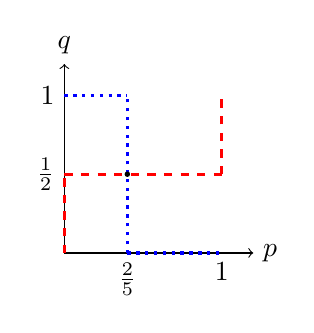
\begin{tikzpicture}[scale=2]
            % Set up the axes
            \draw[->] (0,0) -- (1.2,0) node[right] {$p$};
            \draw[->] (0,0) -- (0,1.2) node[above] {$q$};

            % Add points on axes
            \node[below] at (1,0) {$1$};
            \node[below] at (0.4,0) {$\frac{2}{5}$};
            \node[left] at (0,1) {$1$};
            \node[left] at (0,0.5) {$\frac{1}{2}$};

            % BR2
            \draw[dotted,blue, line width=1.2pt] (0,1) -- (0.4,1);
            \draw[dotted,blue, line width=1.2pt] (0.4,0) -- (1,0);
            \draw[dotted,blue, line width=1.2pt] (0.4,0) -- (0.4,1);

            % BR1
            \draw[dashed,red, line width=1.2pt] (0,0) -- (0,0.5);
            \draw[dashed,red, line width=1.2pt] (0,0.5) -- (1,0.5);
            \draw[dashed,red, line width=1.2pt] (1,0.5) -- (1,1);

            % Add the intersection point
            \fill (0.4,0.5) circle (0.5pt);

        \end{tikzpicture}
    \end{center}
\end{example}
The following enables one to efficiently find (mixed) Nash Equilibria in finite games:
\begin{remark}
    The utility function of one player is \textbf{linear} in its own variable.
\end{remark}
Thus for every (mixed) strategy $y$ of the second player, $\BR_1(y)$ contains at least a pure strategy, since Pl1 maximizes a linear function over a simplex (in fact, such a strategy is a vertex of the simplex). And, likewise, the same holds for Pl2.

\begin{remark}
    Suppose $(\overline{x}, \overline{y})$ is a NE in \textbf{mixed strategies}. Suppose $\spt \overline{x} = \{1, \ldots, k\}$, $\spt \overline{y} = \{1, \ldots, l\}$ and $f(\overline{x}, \overline{y}) = v$. Then:
    \[
        \begin{cases}
            a_{11}\overline{y}_1 + a_{12}\overline{y}_2 + \cdots + a_{1l}\overline{y}_l             & = v    \\
            \vdots                                                                                  & =v     \\
            a_{k1}\overline{y}_1 + a_{k2}\overline{y}_2 + \cdots + a_{kl}\overline{y}_l             & = v    \\
            a_{(k+1)1}\overline{y}_1 + a_{(k+1)2}\overline{y}_2 + \cdots + a_{(k+1)l}\overline{y}_l & \leq v \\
            \vdots                                                                                  & \leq v \\
            a_{n1}\overline{y}_1 + a_{n2}\overline{y}_2 + \cdots + a_{nl}\overline{y}_l             & \leq v
        \end{cases}
    \]

    The above relations follow from the fact that rows with positive probability must be all optimal (and thus they all give the same expected value), while the other rows are suboptimal.
    \begin{note}
        \[
            \spt \overline{x} = \{i \; : \; \overline{x}_i > 0\}
        \]
    \end{note}
    \textit{For Pl2 the same reasoning applies, just with the roles of $a$ and $b$ reversed, and the value $v$ being called $w$}.
\end{remark}
The above system of equalities/inequalities simplifies if one looks for fully mixed Nash equilibria, that is all rows and columns are played with positive probabilities (we call this \textbf{full support}).

Suppose $(\overline{x}, \overline{y})$ is a Nash equilibrium profile. Then it holds that
\[
    a_{i1}\overline{y}_1 + a_{i2}\overline{y}_2 + \cdots + a_{im}\overline{y}_m = a_{k1}\overline{y}_1 + a_{k2}\overline{y}_2 + \cdots + a_{km}\overline{y}_m \qquad \forall i,k = 1, \ldots, n
\]
And similarly for the second player:
\[
    b_{1j}\overline{x}_1 + b_{2j}\overline{x}_2 + \cdots + b_{nj}\overline{x}_n = b_{1l}\overline{x}_1 + b_{2l}\overline{x}_2 + \cdots + b_{nl}\overline{x}_n \qquad \forall j,l = 1, \ldots, m
\]
with the conditions $\sum_{i=1}^n \overline{x}_i = 1$ and $\sum_{j=1}^m \overline{y}_j = 1$.

In this case we apply the \textbf{indifference principle}.
\begin{example}
    On the following game, find $a,b$ such that there is a Nash equilibrium with support in rows 1 and 2 for the first player and columns 2 and 3 for the second player
    \[
        \begin{array}{cccc}
                & 0     & q     & 1-q    \\
            p   & (2,2) & (a,3) & (3,3)  \\
            1-p & (4,0) & (3,4) & (5,b)  \\
            0   & (2,3) & (5,2) & (4,26)
        \end{array}
    \]
    The optimal strategies are $\overline{x} = (p,1-p,0)$ for Pl1 and $\overline{y} = (0,q,1-q)$ for Pl2.

    For the first player one has the following system
    \[
        \underbrace{aq + 3-3q}_{\text{1st row}} = \underbrace{3q + 5 -5q}_{\text{2nd row}} \qquad \underbrace{3q + 5-5q}_{\text{2nd row}} \geq \underbrace{5q +4 -4q}_{\text{3rd row}}
    \]
    Providing respectly the conditions $q = \frac{2}{a-1}$ and $q \leq \frac{1}{3}$, combining the two conditions we get that $a \geq 7$.

    For the second player the first column is strictly dominated, and it must be $b = 4$ (otherwise one column dominates the other one) and in this case every choice of $p \in (0,1)$ works since we have
    \[
        \underbrace{3p+4(1-p)}_{\text{2nd col}} = \underbrace{3p+4(1-p)}_{\text{3rd col}}
    \]
\end{example}
\section{Finite games with common payoff}
Consider a finite game with strategy sets $X_i$ and suppose that all the players have the same payoff $p : X \to \mathbb{R}$, that is for all $i$ the utility functions are
\[
    u_i (x_1, \ldots x_n) = p(x_1, \ldots, x_n) \quad \forall x_i \in X_i
\]
if $\overline{x} = (\overline{x}_1, \ldots, \overline{x}_n)$ is a strategy profile such that $p(\overline{x}) \geq p(x) \quad \forall x \in X$ then $\overline{x}$ is a \textbf{Nash Equilibrium in pure strategies}.
\begin{remark}
    There might be other Nash equilibria in pure or mixed strategies.

    However, $\overline{x}$ is the best strategy for all players.
\end{remark}
Consider the following payoff-improving procedure:
\begin{enumerate}
    \item Start from an arbitrary strategy profile $x = (x_1, \ldots, x_n) \in X$
    \item Ask if any player has a better strategy $x'_i$ that strictly increases her payoff
          \[
              u_i(x'_i, x_{-i}) > u_i(x_i, x_{-i})
          \]
          \begin{itemize}
              \item if yes, replace $x_i$ with $x'_i$ and repeat.
              \item if no, stop, the current strategy profile is a Nash equilibrium!
          \end{itemize}
\end{enumerate}
Each iteration strictly increases the value $p(x)$, so that no strategy profile $x \in X$ can be visited twice. Since $X$ is a finite set, the procedure must reach a pure Nash equilibrium after at most $\abs{X}$ steps.
\begin{remark}
    This procedure guarantees to reach the global maximum $\overline{x}$
\end{remark}
Consider now a arbitrary finite game with payoffs $u_i : X \to \mathbb{R}$. How do best responses and Nash equilibria change, if we add a constant $c_i$ to the payoff of player $i$?
\[
    \tilde{u}_i(x_1, \ldots, x_n) = u_i(x_1, \ldots, x_n) + c_i
\]
What if $c_i$ is not constant but it depends only on $x_{-i}$ and not on $x_i$?
\begin{center}
    \textbf{Best responses and equilibria remain the same!}
\end{center}
The payoffs $\tilde{u}_i$ and $u_i$ are said diff-equivalent for player $i$ , if the difference
\[
    \tilde{u}_i(x_1, \ldots, x_n) - u_i(x_1, \ldots, x_n) = c_i(x_{-i})
\]
does not depend on her decision $x_i$, but only on the strategies of the other players.

By definition, diff-equivalent payoffs are such that for all $\overline{x}_i ,x_i \in X_i$
\[
    \tilde{u}_i(x'_i, x_{-i}) - u_i(x'_i, x_{-i}) = \tilde{u}_i(x_i, x_{-i}) - u_i(x_i, x_{-i}) = c_i(x_{-i})
\]
Denoting $\Delta f(x'_i, x_i, x_{-i}) = f(x'_i, x_{-i}) - f(x_i, x_{-i})$ this can be rewritten as
\[
    \Delta \tilde{u}_i(x'_i, x_i, x_{-i}) = \Delta u_i(x'_i, x_i, x_{-i})
\]
\begin{theorem}
    Finite games with diff-equivalent payoffs have the same pure Nash equilibria.
\end{theorem}
\begin{proof}
    The best reaction multifunction, for every player $i$ , is the same when considering two diff-equivalent payoffs $u_i$ and $\tilde{u}_i$, no matter how different from each other the latter functions are.
\end{proof}
\newpage
\subsection{Potential Games}
\vspace{0.25cm}
\begin{definition}[Potential Game]
    A \underline{finite} game with strategy sets $X_i$ and payoffs $u_i : X \to \mathbb{R}$ is called a potential game, if it is diff-equivalent to a game with common payoffs.

    That is, there exists a \textbf{potential function} $p : X \to \mathbb{R}$ such that for each $i$, for every $x_{-i} \in X_{-i}$, and all $x'_i ,x_i \in X_i$ we have
    \[
        \Delta \tilde{u}_i(x'_i, x_i, x_{-i}) = \Delta p(x'_i, x_i, x_{-i})
    \]
    where $\Delta p(x'_i, x_i, x_{-i}) = p(x'_i, x_{-i}) - p(x_i, x_{-i})$.
\end{definition}
\begin{corollary}\
    \begin{enumerate}
        \item Every \underline{finite} potential game has at least one pure Nash equilibrium
        \item In a \underline{finite} potential game every best response iteration reaches a pure Nash equilibrium in finitely many steps.
    \end{enumerate}
\end{corollary}
\begin{example}
    The game
    \[
        \begin{pmatrix}
            (10,10) & (0,11) \\
            (11,0)  & (1,1)
        \end{pmatrix}
    \]
    has the potential
    \[
        p(x_1, x_2) = \begin{pmatrix}
            0 & 1 \\
            1 & 2
        \end{pmatrix}
    \]
    For Pl1 we have $x_{-1} = x_2$ and thus:
    \begin{itemize}
        \item When the first column is fixed, moving from the first to the second strategy gives $\Delta u_1 = 11-10$, which is equal to $1-0$.
        \item When the second column is fixed, moving from the first to the second strategy gives $\Delta u_1 = 1-0$, which is equal to $2-1$
    \end{itemize}
    For Pl2 we have $x_{-2} = x_1$ and thus:
    \begin{itemize}
        \item When the first row is fixed, moving from the first to the second strategy gives $\Delta u_2 = 11-10$, which is equal to $1-0$.
        \item When the second row is fixed, moving from the first to the second strategy gives $\Delta u_2 = 1-0$, which is equal to $2-1$.
    \end{itemize}
\end{example}
A pontential $p : X \to \mathbb{R}$ is characterized by
\[
    \Delta p (x'_i, x_i, x_{-i}) = \Delta u_i (x'_i, x_i, x_{-i}) \qquad \forall x_i \in X_i, \forall x_{-i} \in X_{-i}
\]
adding a constant to $p(\cdot)$ provides a new potential.

Fix an arbitrary profile $\overline{x} = (\overline{x}_1,\ldots,\overline{x}_n)$ and set $p(\overline{x}) = 0$.

Now the potential $p(\cdot)$ \textbf{is determined uniquely}:
\begin{align*}
    p(x_1, x_2, \ldots, x_n) - p(\overline{x}_1, x_2, \ldots, x_n)                                                     & = u_1(x_1, x_2, \ldots, x_n) - u_1(\overline{x}_1, x_2, \ldots, x_n)                                                     \\
    p(\overline{x}_1, x_2, \ldots, x_n) -p(\overline{x}_1, \overline{x}_2, \ldots, x_n)                                & = u_2(\overline{x}_1, x_2, \ldots, x_n) - u_2(\overline{x}_1, \overline{x}_2, \ldots, x_n)                               \\
                                                                                                                       & \vdots                                                                                                                   \\
    p(\overline{x}_1, \ldots, \overline{x}_{n-1}, x_n) - p(\overline{x}_1, \ldots, \overline{x}_{n-1}, \overline{x}_n) & = u_n(\overline{x}_1, \ldots, \overline{x}_{n-1}, x_n) - u_n(\overline{x}_1, \ldots, \overline{x}_{n-1}, \overline{x}_n)
\end{align*}
By adding all the above equations we get
\[
    p(x_1, x_2, \ldots, x_n) = \sum_{i=1}^n [u_i(\overline{x}_1, \ldots, \overline{x}_{i-1}, x_i, \ldots, x_n) - u_i(\overline{x}_1, \ldots, \overline{x}_{i-1}, \overline{x}_i, \ldots, x_n)]
\]
\begin{note}
    If the game admits a potential the sum on the right hand side of the previous slide is \textbf{independent of the particular order used}.
\end{note}
\begin{example}
    In the following game
    \[
        \begin{pmatrix}
            (2,5) & (2,6) & (3,7) & (8,9) & (5,7) \\
            (1,4) & (1,5) & (3,7) & (2,3) & (0,2) \\
            (6,5) & (2,2) & (0,0) & (6,3) & (3,1)
        \end{pmatrix}
    \]
    The potential is
    \[
        \begin{pmatrix}
            0  & 1 & 2  & 4  & 2  \\
            -1 & 0 & 2  & -2 & -3 \\
            4  & 1 & -1 & 2  & 0
        \end{pmatrix}
    \]
\end{example}
\end{document}